% Figure 4 of article/main_layout.tex: DeCovarT on the Suppinger gastruloids,
% on one portrait A4 page (210 x 297 mm).
%   a  analysis pipeline     DeCovarT_reproducibility/docs/index.qmd (fig-pipeline),
%                            without the optional Fisher / NSGA-II refinement
%   b  design of the series  DeCovarT_reproducibility/docs/01-data-suppinger.qmd
%                            (fig-suppinger-design)
%   c-j                      ggplot2 block from article/scripts/fig04_suppinger.R
%
% Build, from the DeCovarT repository root:
%   Rscript --no-save --no-restore article/scripts/fig04_suppinger.R
%   cd article/scripts && latexmk -lualatex -outdir=../figs fig04_suppinger.tex
%   latexmk -c -outdir=../figs fig04_suppinger.tex
%   cd ../figs && pdftocairo -svg fig04_suppinger.pdf fig04_suppinger.svg
\documentclass[border=0pt]{standalone}
\usepackage{iftex}
\ifPDFTeX
  \PackageError{fig04}{Use LuaLaTeX}{}
\fi
\usepackage{fontspec}
\setmainfont{Noto Sans}
\usepackage{amsmath,amssymb,bm}
\usepackage{graphicx}
\usepackage{xcolor}
\usepackage{tikz}
\usetikzlibrary{arrows.meta,positioning,fit,backgrounds,calc,shapes.geometric}
\graphicspath{{../figs/fig04_suppinger/}}

% Colours of the book's TikZ header (docs/_quarto.yml); ink is the house ink
% of the ggplot2 block, so the page has one text colour.
\definecolor{ink}{HTML}{1C2B24}
\definecolor{latfill}{HTML}{DAE9FB}
\definecolor{latdraw}{HTML}{4477B5}
\definecolor{obsfill}{HTML}{C9CDD3}
\definecolor{obsdraw}{HTML}{747B86}

\hyphenpenalty=10000
\exhyphenpenalty=10000

\newcommand{\sevenpt}{\fontsize{7}{8.4}\selectfont}
\newcommand{\sixpt}{\fontsize{6}{7.2}\selectfont}

% Styles of the book (docs/_quarto.yml), at 7 pt for the A4 page.
\tikzset{
  every node/.style={text=ink},
  box/.style={rectangle, rounded corners=2.5pt, draw=ink, fill=white, line width=0.6pt,
    align=flush center, inner sep=1.2mm, font=\sevenpt},
  keybox/.style={box, draw=latdraw, fill=latfill},
  dimbox/.style={box, draw=obsdraw, fill=obsfill!45},
  note/.style={font=\sixpt, text=ink!80},
  elabel/.style={font=\sixpt\itshape, text=ink!85, fill=white, inner sep=1pt, align=center},
  edge/.style={-{Stealth[length=2mm]}, line width=0.6pt, draw=ink},
  num/.style={font=\sixpt\bfseries, text=ink!70, anchor=south west, inner sep=0.5mm},
  letter/.style={font=\bfseries\fontsize{8}{9.6}\selectfont, anchor=north west, inner sep=0pt},
  pstep/.style={text width=30mm, minimum height=15mm},
}

\begin{document}
\begin{tikzpicture}[x=1mm, y=1mm]
\useasboundingbox (0,0) rectangle (210,297);

% ---------------------------------------------------------------------------
% a. Pipeline: five steps on row 1 (columns at x = 25, 65, ..., 185),
%    three on row 2. Step 6 of the book (optional refinement) is left out
%    and the steps are renumbered.
\node[letter] at (8,289) {a};
\node[dimbox, pstep] (s1) at (25,277) {GSE229513 UMI counts\\ and cell-type labels};
\node[box, pstep] (s2) at (65,277) {Cell and gene QC};
\node[box, pstep] (s3) at (105,277) {Presence gate\\ in every type};
\node[box, pstep] (s4) at (145,277) {Omnibus deviance /\\ quasi-likelihood screen,\\ ranked by effect size};
\node[box, pstep] (s5) at (185,277) {Bulk consistency filter,\\ 48/72/96\,h: single-cell\\ $\leftrightarrow$ standard-Wnt bulk,\\ each matched time};
\node[keybox, text width=70mm, minimum height=15mm] (s6) at (45,256.5) {Per type $\times$ time, linear scale: shrinkage $\widehat{\boldsymbol{\Sigma}}$ (default) $\mid$ glasso $\mid$ SILGGM $\mid$ PLNnetwork;\\ $\lambda$ by cross-validated held-out log-likelihood;\\ nested CV compares the four};
\node[box, pstep] (s7) at (105,256.5) {Lift to DeCovarT moments\\ $\widehat{\boldsymbol{\mu}}_{\cdot j}$, $\widehat{\boldsymbol{\Sigma}}_{W,j}$};
\node[keybox, pstep] (s8) at (145,256.5) {DeCovarT on bulk:\\ standard Wnt,\\ 48/72/96\,h};
\node[note, text width=30mm, align=center] at (185,256.5) {Early Wnt: no matched\\ single-cell reference\\ at any time};
\foreach \k in {1,...,8} {\node[num] at (s\k.north west) {\k};}
\draw[edge] (s1) -- (s2);
\draw[edge] (s2) -- (s3);
\draw[edge] (s3) -- (s4);
\draw[edge] (s4) -- (s5);
\coordinate (turn) at ($(s5.south)!0.5!(s5.south |- s6.north)$);
\draw[edge] (s5.south) -- (turn) -| (s6.north);
\draw[edge] (s6) -- (s7);
\draw[edge] (s7) -- (s8);

% ---------------------------------------------------------------------------
% b. Design of the two GEO series (book coordinates, rescaled to the width).
\node[letter] at (8,246) {b};
\begin{scope}[shift={(23.7,219)}, x=8.7mm, y=6.5mm,
  slot/.style={circle, minimum size=6.2mm, inner sep=0pt, font=\sixpt, line width=0.6pt},
  bulk/.style={rectangle, rounded corners=2pt, draw=ink, fill=white, minimum size=6.4mm,
    inner sep=0.3pt, font=\fontsize{5.5}{6}\selectfont, align=center, line width=0.6pt},
  link/.style={draw=ink, line width=0.6pt}]
% single-cell tree
\node[box] (sc) at (5.8,3.4) {scRNA-seq\\ GSE229513};
\node[box, draw=latdraw, fill=latfill] (bs) at (2.5,1.75) {Cell line B-S};
\node[box, draw=obsdraw, fill=obsfill!60] (sbr) at (9.1,1.75) {Cell line SBR};
\foreach \t [count=\k from 0] in {48,52,56,96,108,120} {
  \node[slot, draw=latdraw, fill=latfill] (bs\t) at (\k,0) {\t};
  \draw[link] (bs.south) -- ++(0,-0.45) -| (bs\t.north);
}
\foreach \t [count=\k from 0] in {24,36,48,60,72,84} {
  \node[slot, draw=obsdraw, fill=obsfill!60] (sbr\t) at (6.6+\k,0) {\t};
  \draw[link] (sbr.south) -- ++(0,-0.45) -| (sbr\t.north);
}
\foreach \n in {bs48,bs96,sbr48,sbr72} {\draw[line width=1.4pt, draw=ink] (\n) circle (3.1mm);}
\draw[link] (sc.south) -- ++(0,-0.5) -| (bs.north);
\draw[link] (sc.south) -- ++(0,-0.5) -| (sbr.north);
\node[note, anchor=east] at (-0.6,0) {time (h)};
% bulk tree
\node[box] (bk) at (16.8,3.4) {Bulk RNA-seq\\ GSE229386};
\node[box] (std) at (15,1.65) {Standard Wnt\\ (pulse at 48\,h)};
\node[box] (early) at (18.6,1.65) {Early Wnt\\ (pulse at 24\,h)};
\foreach \t [count=\k from 0] in {48,72,96} {
  \node[bulk] (std\t) at (14+\k,0) {\t\\[-1pt]×3};
  \draw[link] (std.south) -- ++(0,-0.45) -| (std\t.north);
  \node[bulk] (early\t) at (17.6+\k,0) {\t\\[-1pt]×3};
  \draw[link] (early.south) -- ++(0,-0.45) -| (early\t.north);
}
\draw[link] (bk.south) -- ++(0,-0.3) -| (std.north);
\draw[link] (bk.south) -- ++(0,-0.3) -| (early.north);
\node[note, align=center] at (18.6,-1.15) {no single-cell match};
% matched pairs: 48 h (both lines), 72 h (SBR), 96 h (B-S)
\draw[link, densely dashed] (bs48.south) -- ++(0,-0.75) -| (std48.south);
\draw[link, densely dashed] (sbr48.south) -- ++(0,-0.75);
\draw[link, densely dashed] (sbr72.south) -- ++(0,-1.1) -| (std72.south);
\draw[link, densely dashed] (bs96.south) -- ++(0,-1.45) -| (std96.south);
\node[elabel] at (11.8,-0.98) {matched pairs, 48/72/96\,h};
% legend, top left (free space beside the single-cell tree)
\node[slot, draw=latdraw, fill=latfill, minimum size=3mm] at (-1,3.55) {};
\node[note, anchor=west] at (-0.75,3.55) {B-S};
\node[slot, draw=obsdraw, fill=obsfill!60, minimum size=3mm] at (0.3,3.55) {};
\node[note, anchor=west] at (0.55,3.55) {SBR};
\node[slot, draw=ink, minimum size=3mm] at (1.6,3.55) {};
\node[note, anchor=west] at (1.85,3.55) {single-cell slot};
\node[bulk, minimum size=3mm] at (-1,2.85) {};
\node[note, anchor=west] at (-0.75,2.85) {bulk time point, 3 biological replicates};
\end{scope}

% ---------------------------------------------------------------------------
% c-j. ggplot2 block (cowplot), written at 194 x 195 mm by the R script.
\node[anchor=south west, inner sep=0pt] at (8,8) {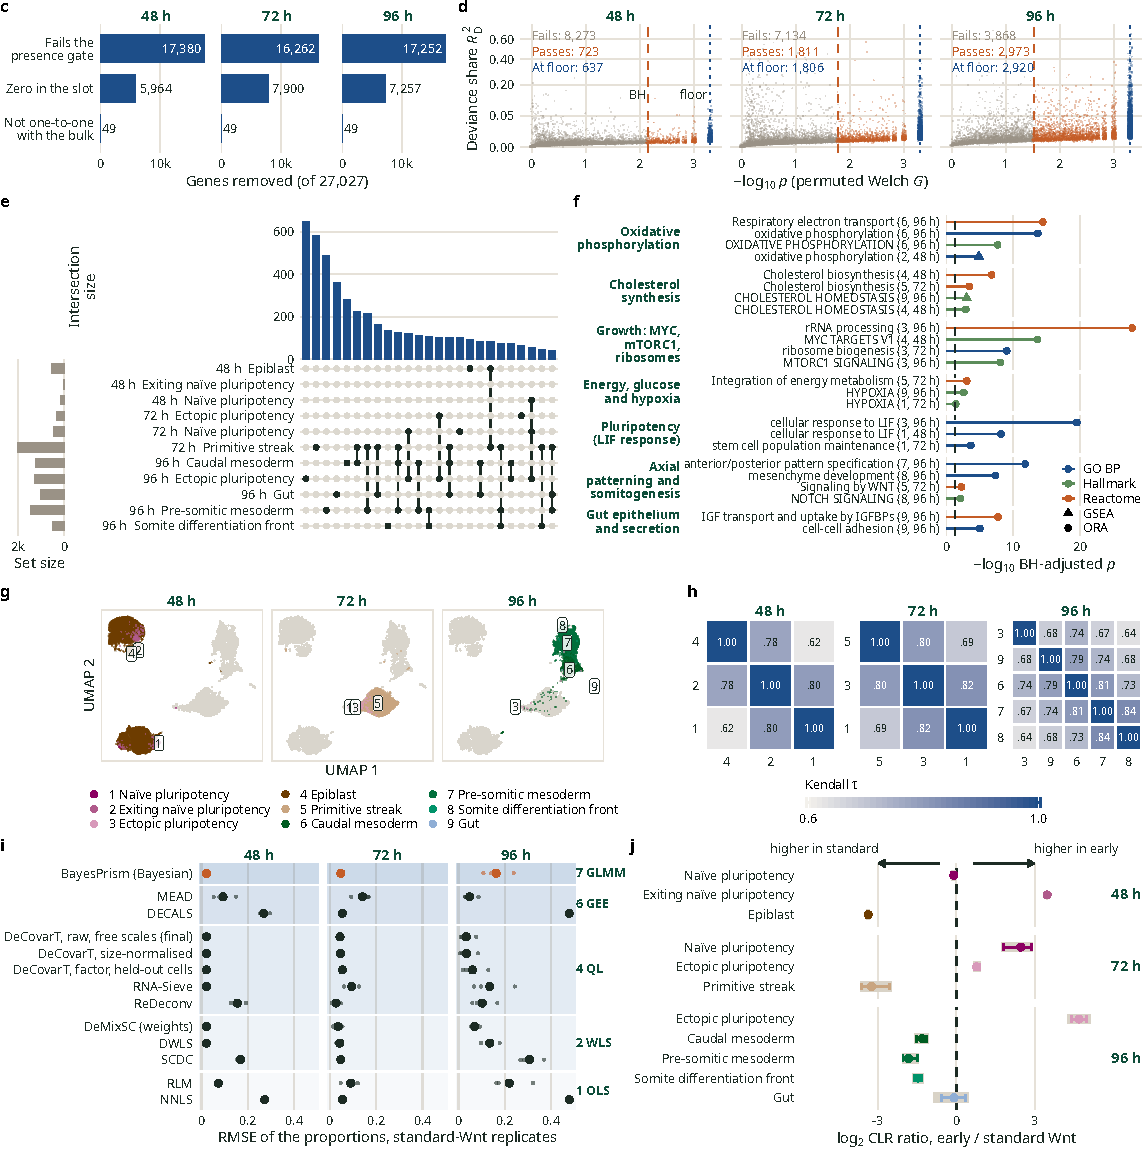
\includegraphics{panel_block.pdf}};
\end{tikzpicture}
\end{document}
